% ============================================================
% IEEE Transactions on Human-Machine Systems (THMS)
% Main manuscript
% ============================================================

\documentclass[journal]{IEEEtran}

\usepackage[T1]{fontenc}
\usepackage{amsmath,amssymb}
\usepackage{newtxtext,newtxmath}
\usepackage[final]{microtype}
\usepackage{graphicx}
\usepackage{cite}
\usepackage{booktabs}
\usepackage{tabularx}
\usepackage{array}
\usepackage{url}
\usepackage[hidelinks]{hyperref}

\newcolumntype{Y}{>{\raggedright\arraybackslash}X}
\graphicspath{{figures/}}

\title{From Nominal Conditions to Realized Interventions:\\
A Fidelity Framework for Asynchronous Human--Machine Experiments}

\author{Fengjie~Ma\textsuperscript{a},
Chuang~Cao\textsuperscript{b},
Qixin~Cao\textsuperscript{b},
Yilin~Zhou\textsuperscript{a},
and~Hua~Zhang\textsuperscript{a,*}%
\thanks{\textsuperscript{a}School of Mechanical and Automotive Engineering,
Shanghai University of Engineering Science, 333 Longteng Road, Shanghai
201620, China.}%
\thanks{\textsuperscript{b}School of Mechanical Engineering, Shanghai Jiao
Tong University, 800 Dongchuan Road, Shanghai 200240, China.}%
\thanks{*Corresponding author: Hua Zhang
(e-mail: \href{mailto:huazhang@yeah.net}{huazhang@yeah.net}).}%
\thanks{Ethics approval or exemption and informed-consent procedures must be
resolved from contemporaneous institutional records:
[ETHICS RECORD REQUIRED---DO NOT SUBMIT].}}

\begin{document}

\maketitle

\begin{abstract}
Asynchronous visual, haptic, and control interventions can alter the machine
states available to an operator during an outcome window. Condition labels
alone do not establish what was actually delivered and exposed in
the operator--machine loop. We propose a realized-intervention fidelity
framework that links the nominal specification, executable implementation,
trial-level realized intervention, and outcome as
$N_m\rightarrow C_m\rightarrow R_i\rightarrow Y_i$, while representing the
closed-loop response pathway as
$R_i(t)\rightarrow H_i(t+\delta)\rightarrow R_i(t+\delta)\rightarrow Y_i$.
The framework reconstructs a five-field evidence state from specifications,
source code, events, state trajectories, and
acquisition provenance. Outcome-blind deterministic rules then constrain the
identity of scientifically supportable comparisons. We applied the framework
to 180 trials from 5 participants in an archived bilateral teleoperation
system. For G, a post-contact nominal specification was not recoverable, and
activation preceded recorded contact in 43/45 trials. For F, the nominal
post-contact 0.20-s guard contained a clock-domain mismatch, and only 3/45
trials met that timing. For E, visual-configuration exposure during the
post-contact 0.20--1.00-s window was full in 39 trials, partial in 2, and zero
in 4. These findings recast the proposed G, F, and interaction comparisons as
realized-configuration comparisons with explicit timing, bundled components,
and exposure distributions. In the retained exploratory E--A comparison, the
mean operational excess-force impulse difference was $-0.3489$~N$\cdot$s,
with a consistent direction across 5/5 participants. With $n=5$, this pattern
does not provide confirmatory causal evidence for an isolated component. The
framework identifies what was delivered and exposed in the loop and what can
be scientifically compared.
\end{abstract}

\begin{IEEEkeywords}
Asynchronous control, evidence provenance, experimental validity,
human--machine systems, implementation fidelity, realized intervention,
teleoperation.
\end{IEEEkeywords}

% ============================================================
\section{Introduction}
% ============================================================

\IEEEPARstart{T}{eleoperation}, shared control, and other closed-loop
human--machine experiments commonly define experimental conditions as fixed,
adaptive, vision-enabled, force-feedback, or combined modes
\cite{hannaford1989,lawrence1993,hokayem2006,passenberg2010,huang2019,rakita2020,louca2024,gong2024,hogan1985,walker2010,buchli2011,ajoudani2012,peternel2018,abudakka2018,abudakka2020,michel2021,peternel2023,michel2023,huang2021,siegemund2024}.
These labels facilitate assignment and reporting, but they do not establish
that the corresponding intervention was delivered in every trial with the
intended guards, clocks, parameters, and duration in the operator--machine
loop. Asynchronous vision processes, control updates, contact detection, and
logging channels can alter intervention onset, duration, and coverage of the
outcome window. ``Post-contact,'' ``vision-enabled,'' and ``vision + force''
are therefore experimental commitments that must first be verified, rather
than established trial-level facts.

% Reference 21 is retained in its source-list position although it is not cited
% in the approved manuscript prose.
\nocite{jekel2026}

This distinction has direct scientific consequences in human--machine
systems. After the realized intervention $R_i(t)$ changes the visual, haptic,
or machine state, the operator may update subsequent input $H_i(t+\delta)$.
This update can change the subsequent machine realization and the complete
outcome trajectory:
\begin{equation}
R_i(t)\rightarrow H_i(t+\delta)\rightarrow R_i(t+\delta)\rightarrow Y_i.
\label{eq:closed_loop}
\end{equation}
An intervention that begins 0.8~s early is therefore not merely a software
parameter written ahead of schedule. The operator may receive different
feedback during approach, contact, or closed-loop correction, producing a
different human--machine trajectory. If outcomes are compared only by nominal
condition labels, the resulting statistic may precisely describe a set of
data without answering the stated human--machine intervention question.

Prior work has separately established the importance of transparency and
latency in teleoperation \cite{hannaford1989,lawrence1993,hokayem2006,passenberg2010,huang2019,rakita2020,louca2024,gong2024},
variable impedance and teleimpedance
\cite{hogan1985,walker2010,buchli2011,ajoudani2012,peternel2018,abudakka2018,abudakka2020,michel2021,peternel2023,michel2023,huang2021,siegemund2024},
visual--haptic timing \cite{vogels2004}, reproducibility in human--machine
research \cite{bonsignorio2015,bonsignorio2017,gunes2022,aldana2023,bagchi2023,marchesi2024},
runtime verification \cite{huang2014}, implementation fidelity
\cite{carroll2007}, and estimand definition \cite{lundberg2021}. HRI-specific
work also provides guidance for experimental design and logging
\cite{hoffmanZhao2020}, common task-oriented and collaborative-fluency metrics
\cite{steinfeld2006,hoffman2019}, formal guarantees for interactive robots
\cite{kressGazit2021}, and validation of synchronization in time-sensitive
robot logs \cite{vigni2024}. A joint layer is still needed before statistical
analysis. It must determine whether
a nominal intervention is supported by a specification, whether the
implementation encodes that specification, what was actually delivered in
each trial, how much exposure occurred within the outcome window, and whether
the intervention can be linked exactly to the analyzed record.

This article addresses three research questions:
\begin{itemize}
    \item \textbf{RQ1 (Reconstructability):} Can realized-intervention
    fidelity be reconstructed from archived specifications, source code,
    events, trajectories, and provenance without using outcome values,
    directions, or significance?
    \item \textbf{RQ2 (Realized discontinuities):} What discontinuities arise
    among the nominal specification, executable implementation, realized
    delivery, and window exposure in an operational asynchronous teleoperation
    system?
    \item \textbf{RQ3 (Comparison identity):} How does realized-intervention
    reconstruction change the condition comparisons that the available data
    can scientifically support?
\end{itemize}

This article makes three contributions. First, it formulates
realized-intervention fidelity as a distinct evaluation layer for asynchronous
human--machine experiments, making the intervention actually delivered and
exposed in the loop an object that must be verified before statistical
comparison. Second, it operationalizes this layer through auditable evidence
states and deterministic interpretation constraints. Without examining human
outcomes, these constraints distinguish identity retention, an unrecoverable
nominal specification, implementation or delivery mismatches, and incomplete
exposure. Third, the framework is applied to an archived teleoperation system
and shows how reconstruction can materially recast nominal factorial claims as
narrower comparisons among realized configurations. The case study is not
interpreted as external validation of the framework, and passing a fidelity
assessment is not treated as a substitute for the conditions required for
causal identification.

\begin{figure*}[t]
    \centering
    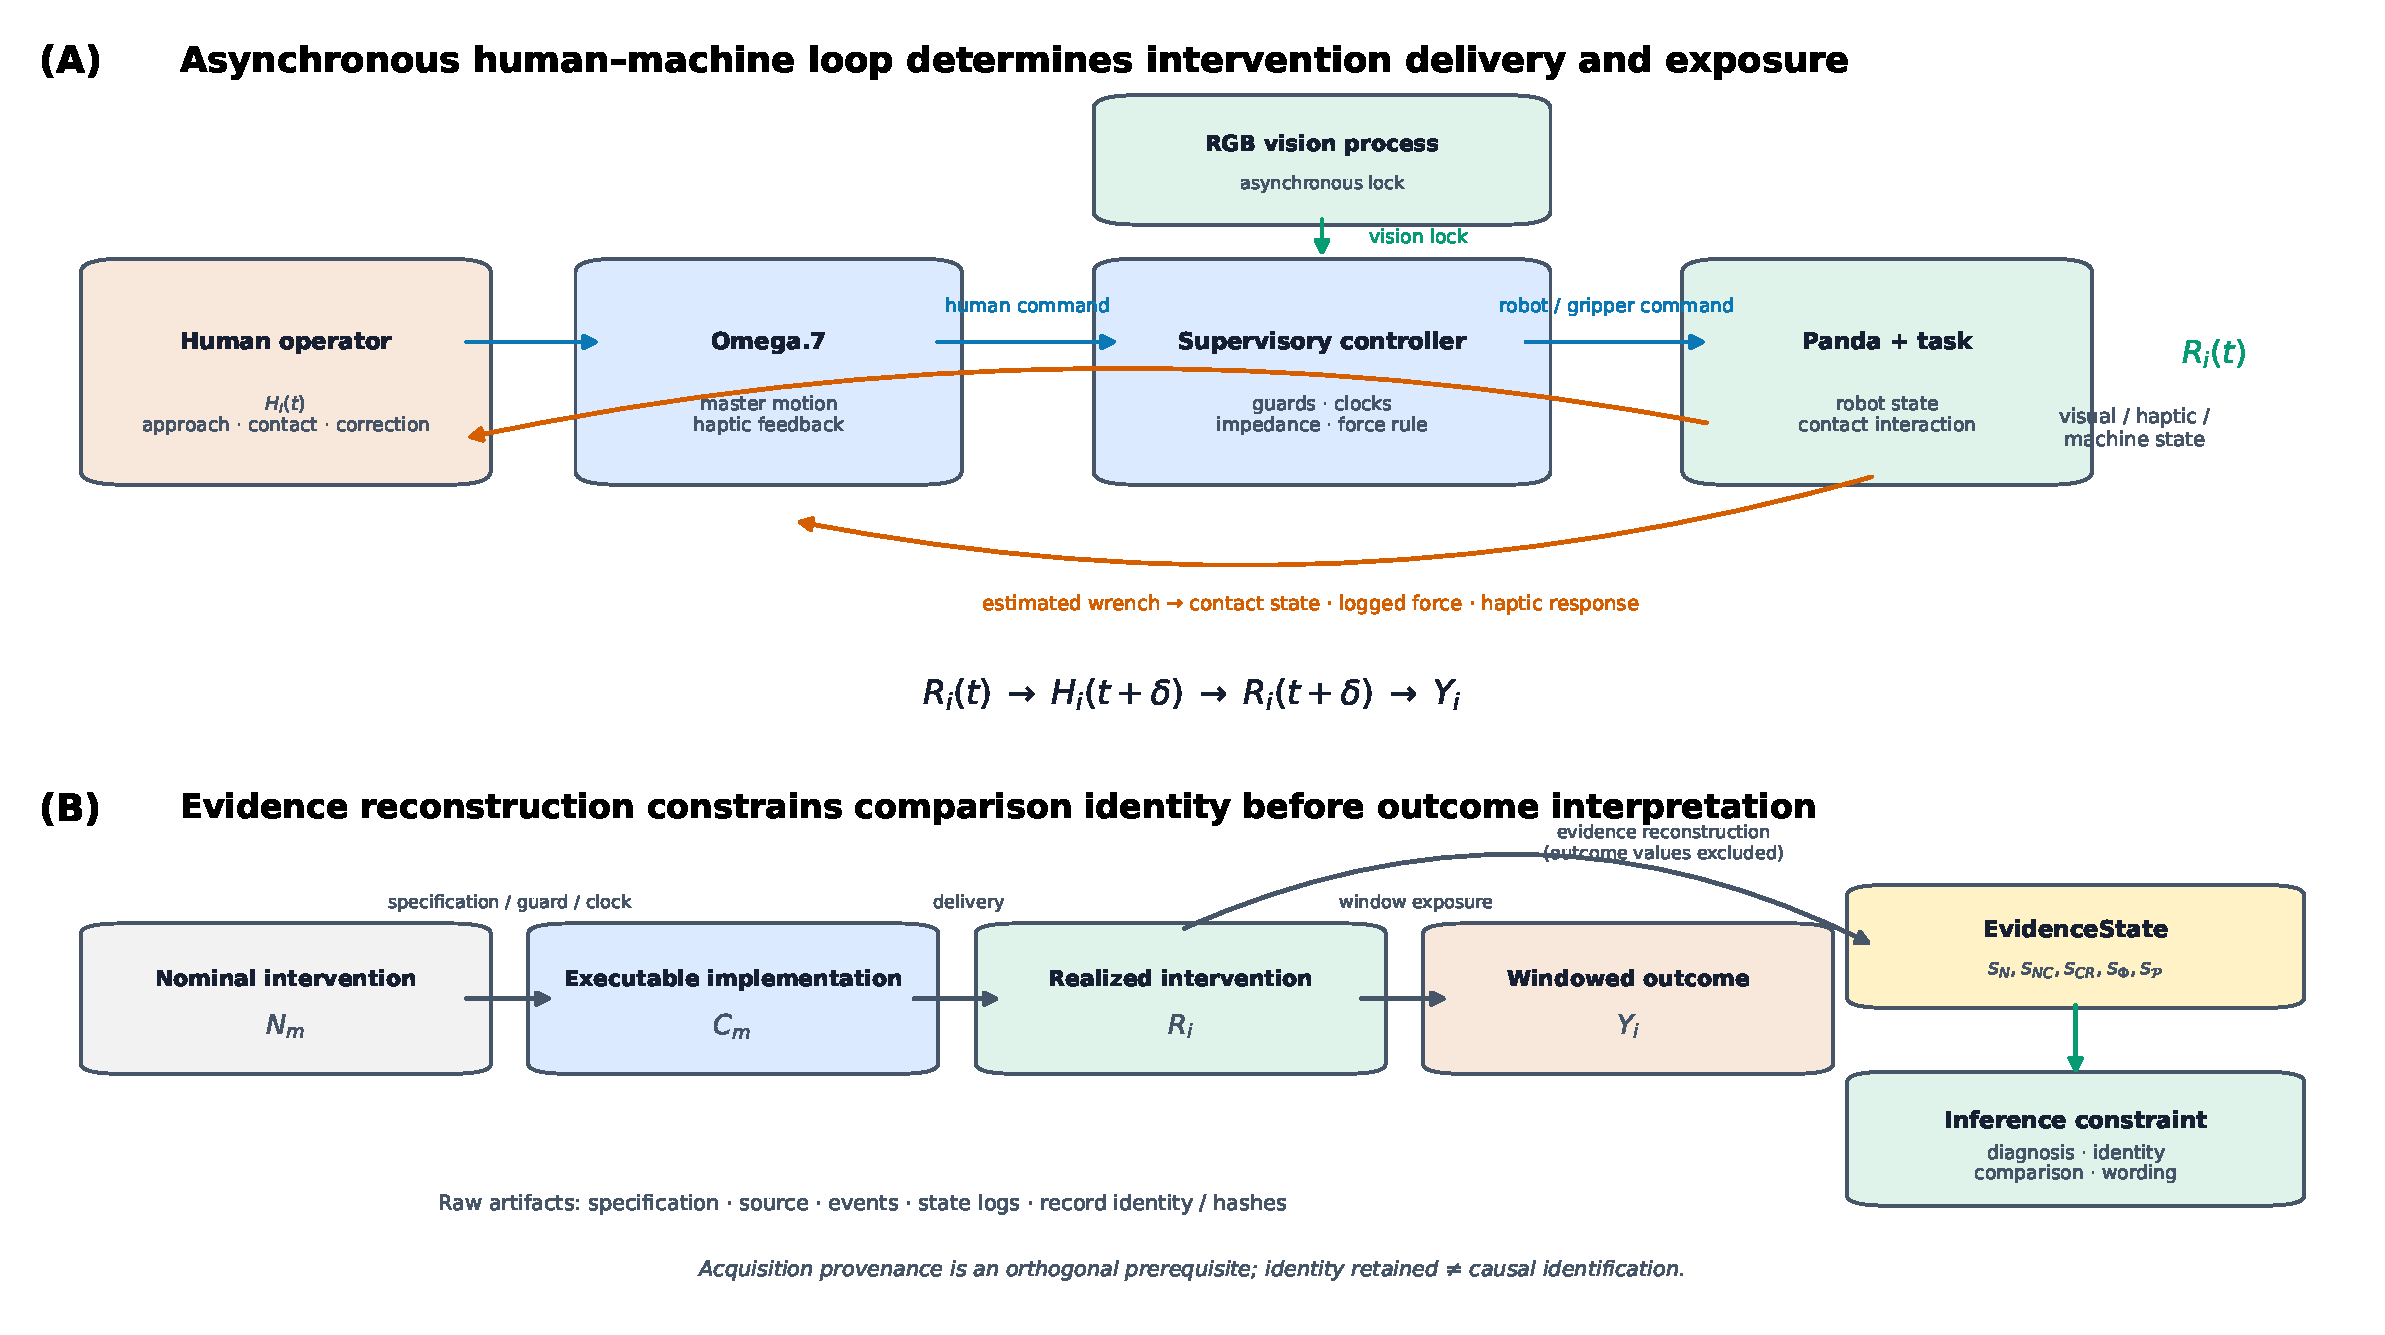
\includegraphics[width=0.98\textwidth]{Fig01_human_machine_fidelity_framework_v5_1.pdf}
    \caption{Asynchronous human--machine loop and the realized-intervention
    fidelity framework. (A) The operator, Omega.7, asynchronous
    vision/supervisory controller, Panda, and haptic and machine-state feedback
    form a closed loop; intervention timing can change subsequent human input
    and the outcome trajectory. (B) The $N\rightarrow C\rightarrow R\rightarrow
    Y$ evidence chain supported by contemporaneous artifacts is reconstructed
    as an evidence state, which then constrains comparison identity and
    scientifically admissible wording. Provenance is an orthogonal prerequisite
    for linking realized interventions to outcomes; retention of identity does
    not imply causal identification.}
    \label{fig:framework}
\end{figure*}

% ============================================================
\section{Related Work}
% ============================================================

\subsection{Timing and Intervention Exposure in Closed-Loop Teleoperation}

Research on bilateral teleoperation has long examined stability,
transparency, communication latency, and feedback quality
\cite{hannaford1989,lawrence1993,hokayem2006,passenberg2010,huang2019,rakita2020,louca2024,gong2024}.
Variable-impedance, teleimpedance, and vision-assisted approaches further
allow controllers to adapt robot responses online according to the task,
environment, or operator state
\cite{hogan1985,walker2010,buchli2011,ajoudani2012,peternel2018,abudakka2018,abudakka2020,michel2021,peternel2023,michel2023,huang2021,siegemund2024}.
This literature shows that visual, haptic, and machine dynamics jointly shape
human control behavior. Outcome analyses in many human--machine experiments
are organized by assigned condition, whereas trial-level intervention
delivery and window exposure are not the primary objects of evaluation.
Research on visual--haptic timing also indicates that people can detect
relatively small cross-modal temporal discrepancies \cite{vogels2004}. This
finding motivates closer attention to realized onset timing but does not, by
itself, reconstruct each intervention in archived trials.

\subsection{Reproducibility, Runtime Evidence, and Implementation Fidelity}

Research in robotics and human--robot interaction has emphasized transparency
in artifacts, code, procedures, and experimental units
\cite{bonsignorio2015,bonsignorio2017,gunes2022,aldana2023,bagchi2023,marchesi2024}.
HRI experiment-design guidance recommends retaining study records and computer
logs for later review \cite{hoffmanZhao2020}. Work on HRI dataset reliability
further shows that synchronization between temporally sensitive robot records
and annotations must itself be checked \cite{vigni2024}.
Runtime verification can monitor formal software properties \cite{huang2014},
whereas implementation-fidelity research distinguishes planned interventions
from their implementation \cite{carroll2007}. Both provide important
foundations for this study, but neither alone determines the comparison
identity of a human--machine experiment. Satisfying a software property does
not establish that the operator received full exposure during the outcome
window. Conversely, an observed state in a log cannot restore a missing
scientific specification.

Related HRI work has also organized task-oriented system measures
\cite{steinfeld2006} and objective and subjective measures of collaborative
fluency \cite{hoffman2019}. These contributions clarify what should be
measured, whereas the present framework asks whether the intervention identity
underlying such a measure is supported at the trial level. Formal-methods
research has similarly articulated verification, validation, and synthesis
challenges for HRI systems \cite{kressGazit2021}. The additional step here is
to transform archived intervention evidence into a scientifically admissible
comparison identity.

Work on estimands emphasizes alignment among the theoretical question, the
comparison, and the statistical quantity \cite{lundberg2021}. Accordingly,
this study does not create a new causal target after observing the realized
intervention. Instead, the evidence chain is used to constrain the narrowest
supportable descriptive comparison. The methodological gap is not the absence
of another fidelity score, but the absence of an operational transformation
from ``specification--implementation--realized delivery--window
exposure--record identity'' to ``what comparisons are admissible.''

% ============================================================
\section{Realized-Intervention Fidelity Framework}
% ============================================================

\subsection{From the Human--Machine Loop to the Evidence Chain}

The evidence chain for one comparison in a human--machine experiment, shown
in Fig.~\ref{fig:framework}(B), is represented as
\begin{equation}
N_m\rightarrow C_m\rightarrow R_i\rightarrow Y_i,
\label{eq:evidence_chain}
\end{equation}
where $N_m$ is the nominal intervention supported by contemporaneous
artifacts, $C_m$ is the executable implementation in the archived acquisition
program, $R_i$ is the realized intervention recorded in trial $i$, and $Y_i$
is the outcome defined over a frozen window and experimental unit. Acquisition
provenance $\mathcal{P}_i$ is an orthogonal prerequisite for linking $R_i$ to
$Y_i$; it is not part of the intervention itself.

\subsection{Five Evidence Questions}

The framework represents evidence as a five-field state:
\begin{equation}
S=(s_N,s_{NC},s_{CR},s_{\Phi},s_{\mathcal{P}}).
\label{eq:evidence_state}
\end{equation}
The five fields address the following scientific questions:
\begin{enumerate}
    \item $s_N$: Is the intervention originally intended for delivery in the
    operator--machine loop known?
    \item $s_{NC}$: Does the archived implementation encode an intervention
    supported by contemporaneous artifacts?
    \item $s_{CR}$: Do the recorded inputs and trajectories support that the
    implementation was actually delivered?
    \item $s_{\Phi}$: Did the intervention occur within the frozen outcome
    window, and how much of the window did it cover?
    \item $s_{\mathcal{P}}$: Can the intervention trajectory be linked exactly
    to the outcome record being analyzed?
\end{enumerate}

States are derived either by automated computation or by a structured author
audit. Automated computation is used for event differences, trajectories,
exposure, identity, and hashes. The structured audit evaluates whether
contemporaneous artifacts constitute an adequate specification and whether
the specification corresponds semantically to the source code. No independent
dual-review semantic audit was performed; inter-rater agreement is therefore
not reported. Complete field definitions, rules, tolerances, missing-data
handling, and source audits are provided in Supplementary Tables S1--S4.

For a binary activation state $a_i(t)$ and a window $W=[t_0,t_1]$, exposure is
defined as
\begin{equation}
\Phi_i(W)=\frac{1}{|W|}\int_{t_0}^{t_1}\mathbb{I}[a_i(t)=1]\,dt.
\label{eq:exposure}
\end{equation}
Full, partial, and zero exposure are encoded using frozen numerical
boundaries. If the trajectory or window is incomplete, exposure is recorded
as unavailable rather than replaced with zero.

\subsection{From Evidence State to Admissible Interpretation}

Evidence states are not aggregated into a single score. Instead, they
determine the diagnosis, intervention identity, admissible comparison level,
and prohibited wording. The main text uses four interpretation boundaries: an
intact identity chain, a nominal specification that is not recoverable, an
implementation/delivery mismatch, and incomplete exposure. An operational
summary is provided in Table~\ref{tab:interpretation}; the complete
deterministic rules are provided in Supplementary Table S2.

The decision logic is hierarchical rather than compensatory. A downstream
pass cannot repair an upstream identity break: replay-consistent delivery
does not recover a missing nominal specification, and observed window
exposure does not establish complete $C\rightarrow R$ fidelity. Conversely, a
not-evaluable field does not erase what can be reconstructed directly; timing
and exposure may remain reportable while the corresponding delivery claim is
withheld. Provenance is a gating requirement: if $R_i$ and $Y_i$ cannot be
linked to the same record, intervention--outcome evaluation stops. Multiple
diagnoses may therefore coexist, and the admissible comparison is bounded by
the weakest evidence-supported link.

When the nominal identity cannot be retained, a descriptive comparison
between realized configurations can be reported:
\begin{equation}
D^R_{m_1,m_0}=\mathbb{E}[Y\mid R\in\mathcal{R}_{m_1}]
-\mathbb{E}[Y\mid R\in\mathcal{R}_{m_0}].
\label{eq:realized_comparison}
\end{equation}
$D^R$ is not a causal target redefined after observing $R$. Any causal
interpretation still requires additional support for the assignment
mechanism, exchangeability, consistency, measurement validity, and
independent units of inference.

% ============================================================
\section{Archived Human--Machine Experiment and Reconstruction Methods}
% ============================================================

\subsection{Human Teleoperation System and Experimental Structure}

The archived system comprised an Omega.7 human input device, a Franka Panda
robot with a Franka Hand, an Intel RealSense D435i RGB vision process, a
supervisory controller, impedance/force-feedback updates, and asynchronous
logs. The operator commanded master-device motion through the Omega.7. The
supervisory controller combined visual locking, contact estimation, and
configuration logic to generate machine commands. External force estimated
internally by the Panda contributed both to contact-related states and,
through the force-feedback channel, to operator input. This architecture
formed a closed loop in which visual, haptic, and machine states acted jointly.

The 5 participants completed 180 analyzed trials across 3 materials, 3
repeated blocks, and 4 configurations, with 45 trials per configuration.
Repeated trials were used to describe trial-level fidelity, but the
participant remained the independent human experimental unit for outcome
analysis ($n=5$). Participant demographics, training, object geometry, and
prospective randomization or counterbalancing were not recovered from the
current record lineage.

\begin{figure*}[t]
    \centering
    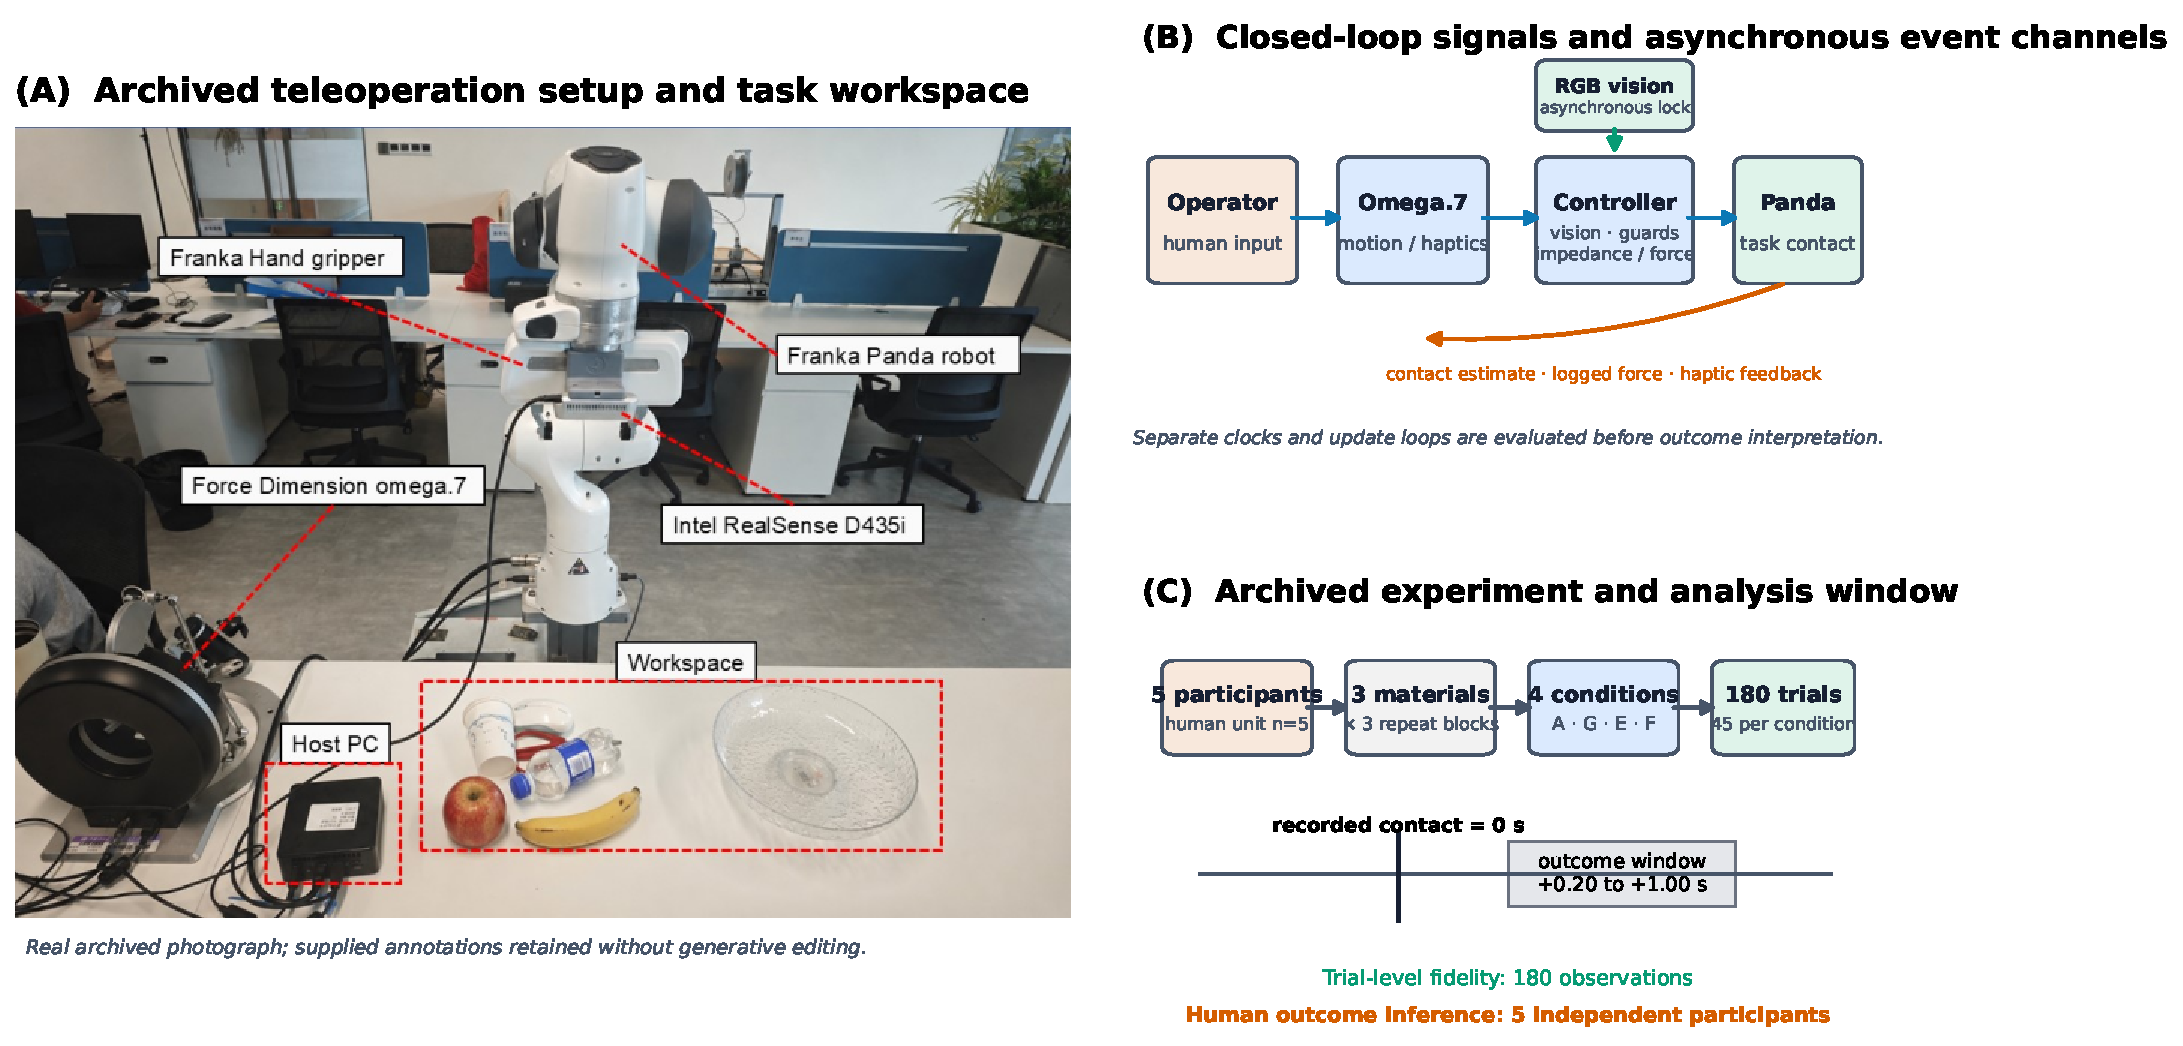
\includegraphics[width=0.98\textwidth]{Fig02_system_experiment_v5_1.pdf}
    \caption{Experimental apparatus, closed-loop signal paths, and archived
    experimental procedure. (A) Physical experimental apparatus, including
    the Omega.7, Panda, Franka Hand, RealSense, and task workspace. (B)
    Closed-loop signals and asynchronous event channels. (C) Archived
    experimental structure and outcome window. The figure describes only the
    system and measurement procedure; it does not report reconstruction
    results.}
    \label{fig:system}
\end{figure*}

\subsection{Archived Conditions and Intended Operator-Side Exposure}

The four archived configurations were labeled A, G, E, and F. Table
\ref{tab:conditions} reports only the experimental structure recoverable from
condition definitions and program documentation. ``Intended operator-side
exposure'' is not inferred from a label; final identity is determined by
framework-based reconstruction.

\begin{table*}[t]
\caption{Archived Experimental Conditions and Operator-Side Exposures to Be Verified}
\label{tab:conditions}
\centering
\scriptsize
\begin{tabularx}{\textwidth}{@{}p{0.055\textwidth}p{0.19\textwidth}p{0.20\textwidth}Yp{0.20\textwidth}@{}}
\toprule
Config. & Primary channels and machine changes & Trigger or timing indicated by labels/artifacts & Operator-side exposure to be verified & Evaluation prerequisite \\
\midrule
A & Fixed impedance and fixed command configuration & Remains fixed after initialization & Fixed machine response and force-feedback baseline & Verify initialization and trial trajectory \\
G & Original online force rule without vision & Label suggests a contact-related adjustment & Force-related change in machine response; the specific ``post-contact'' meaning cannot be established from the label alone & Recover an independent specification and replay the rule \\
E & Visual lock triggers a bundled multiparameter configuration & Transition after the first valid visual lock & Bundled machine and haptic changes delivered after visual recognition & Verify mapping, transition, and window exposure \\
F & Force refinement added to E & Artifacts indicate gating at 0.20~s after contact & Exposure first to the bundled visual change and then to delayed force refinement & Verify guard, clock, delivery, and exposure \\
\bottomrule
\end{tabularx}
\end{table*}

\subsection{Evaluation Rules and Realized-Intervention Reconstruction}

\begin{table*}[t]
\caption{Evidence Scenarios and Admissible Scientific Interpretations}
\label{tab:interpretation}
\centering
\scriptsize
\begin{tabularx}{\textwidth}{@{}p{0.24\textwidth}Y Y@{}}
\toprule
Evidence scenario & Supportable interpretation & Unsupported claim \\
\midrule
Identity chain intact and provenance valid & Retain the nominal intervention identity supported by the specification & Claim a causal effect from fidelity alone \\
Nominal specification not recoverable & Describe the recoverable realized configuration and exposure & Interpret a condition label as the unrecovered nominal intervention \\
Implementation or delivery mismatch / not fully evaluable & Describe the recorded implementation, trajectory, or delivery state & Claim that the intended strategy or $C=R$ has been established \\
Window exposure partial, zero, or unavailable & Provide an assignment-based description qualified by the exposure distribution, or stop the corresponding evaluation & Claim a uniformly complete intervention effect within the window \\
\bottomrule
\end{tabularx}
\end{table*}

All trials point to acquisition commit
\texttt{09c13e0b679905f14f770d820af00841546cb4cc}. Configuration-level semantic
audits used the source-code snapshot from that commit. Trial-level automated
computations used the master manifest, raw CSV files, event JSON files,
summary JSON files, logged states, and current SHA-256 hashes.

For each configuration, reconstruction sequentially examined the
contemporaneous specification; the guards, clocks, parameters, initialization,
and update logic in the source code; state or command trajectories under
recorded inputs; left-continuous exposure within the frozen window; and the
links among logical trial, acquisition record, and file hash. When complete
replay was possible, recorded inputs were supplied to archived formulas and
the results were compared with logged trajectories. When cycle-level
predicate inputs were missing, delivery fidelity was conservatively recorded
as not evaluable, while directly reconstructable activation and exposure
descriptions were retained. Any missing specification, implementation
mismatch, unavailable replay, or incomplete exposure was encoded before
outcomes were examined.

Reconstruction separated trial-level quantities from comparison-level
identity. The former comprised activation time, exposure, trajectory, and
record linkage; the latter followed only after applying the frozen rules to
the collection of trial states and the configuration-level semantic audit.
With left-continuous reconstruction, a logged transition contributed exposure
only from its recorded occurrence forward. Repeated trials improved the
description of delivery heterogeneity but neither created additional human
units nor authorized outcome-dependent regrouping.

When both target activation $t^N_{\mathrm{act}}$ and a common clock mapping
were supported, timing error was defined as
\begin{equation}
\epsilon_{\mathrm{act}}=t^R_{\mathrm{act}}-t^N_{\mathrm{act}}.
\label{eq:timing_error}
\end{equation}
The clock-domain check compared the sources and origins of time values on the
two sides of the guard; trial timing was described using aligned recorded
events. The method did not infer an unknown nominal specification from
recorded activation times, nor did it attribute an outcome jointly produced by
scheduling, other guards, and log sampling to a single software expression.

\subsection{Outcome and Statistical Analysis}

The primary outcome was operational above-threshold force impulse during the
post-contact 0.20--1.00-s window. This window corresponds to the stage in
which the operator enters post-contact closed-loop correction and subsequent
input can be affected by visual, haptic, and machine-impedance states. Both
contact alignment and impulse calculation used the Panda internal
\texttt{O\_F\_ext\_hat\_K} estimate. The outcome was therefore an operational
contact outcome measured within the human--machine loop, rather than a physical
safety endpoint measured by an independent external force sensor.

Data were first aggregated within material and repeated block for each
participant, after which paired configuration differences were calculated. We
report the participant mean, t-based 95\% confidence interval, paired t-test,
exact sign-flip test, exact Wilcoxon test, and Holm correction across 4
comparisons. With only 5 participants, the outcome analysis remained an
exploratory illustration. Record-selection robustness enumerated all
$2^6=64$ choices across 6 initial/alternative record pairs. Fixed adjacent
windows, leave-one-participant-out analyses, and secondary timing metrics are
retained in the Supplementary Material.

\subsection{Rule-Level Internal Verification}

The two-stage interface was implemented as
\texttt{ArtifactEvidence}$\rightarrow$\texttt{EvidenceState} and
\texttt{EvidenceState}$\rightarrow$\texttt{Decision}. Inputs, expected states,
and expected decisions were stored in a frozen oracle table separate from the
executable code. The 12 controlled artifact cases covered an intact chain, a
missing specification, guard/clock mismatches, runtime deviations,
partial/zero/unavailable exposure, invalid provenance, and multiple
co-occurring discontinuities. This check tested only whether the implementation
faithfully executed the stated rules and could be challenged by
counterexamples. It did not estimate sensitivity to unknown faults,
completeness of the state space, or cross-system validity.

Cases were chosen to exercise decision boundaries and distinct missingness
states rather than to approximate their prevalence. Each case had frozen
expected intermediate states as well as a final decision, so disagreement
could be localized to evidence extraction or interpretation. Cases with
co-occurring breaks tested cumulative diagnoses and the precedence of gating
rules. Passing these cases establishes conformance to the declared rule table,
not the scientific completeness of that table.

% ============================================================
\section{Results}
% ============================================================

\subsection{RQ1--RQ2: Realized Timing and Exposure in Operational Trials}

All 180/180 intervention trajectories were linked to outcomes through checks
of exact record identity, path, timestamp, acquisition commit, and current
hash. The executable original force rule for G was replayable at 12,196 logged
command updates across 45 trials. The maximum numerical errors for force
ratio, target translational stiffness, and the 0.3 smoothing update were all
below $10^{-10}$. However, an independent contemporaneous artifact could not
recover the nominal ``post-contact G'' specification, and G activated before
recorded contact in 43/45 trials. Delivery consistency with the source-code
equation therefore cannot restore the missing scientific intent.

The F source code passed \texttt{time.time()} into a system-time calculation
whose origin was \texttt{time.perf\_counter()}, thereby violating the clock
semantics of the nominal 0.20-s post-contact guard. F never activated before
contact, but only 3/45 trials activated at least 0.20~s after contact; the
observed median contact-to-activation interval was 0.05327~s. This recorded
interval of approximately 53~ms resulted from the complete downstream path,
including other guards, scheduling, state conditions, and log sampling. It was
not a 53-ms delay numerically ``caused'' by the mixed-clock expression.
Activation and exposure for F could be reconstructed, but complete cycle-level
predicate inputs were unavailable. Accordingly, $s_{CR}$ was recorded as
\texttt{not\_evaluable}, rather than \texttt{pass} or \texttt{fail}.

Exposure to the visual configuration for E within the outcome window was full
in 39 trials, partial in 2, and zero in 4. In the 4 zero-exposure trials, both
visual lock and completion of the transition occurred after the end of the
window. The two partial-exposure values were 0.966863 and 0.00115488; the
latter covered only approximately 1~ms at the end of the window. For F,
exposure to the visual configuration was full in 42 trials and zero in 3.
Exposure to the force adaptation and joint visual--adaptation configuration
was full in 35 trials, partial in 7, and zero in 3.

\begin{figure*}[t]
    \centering
    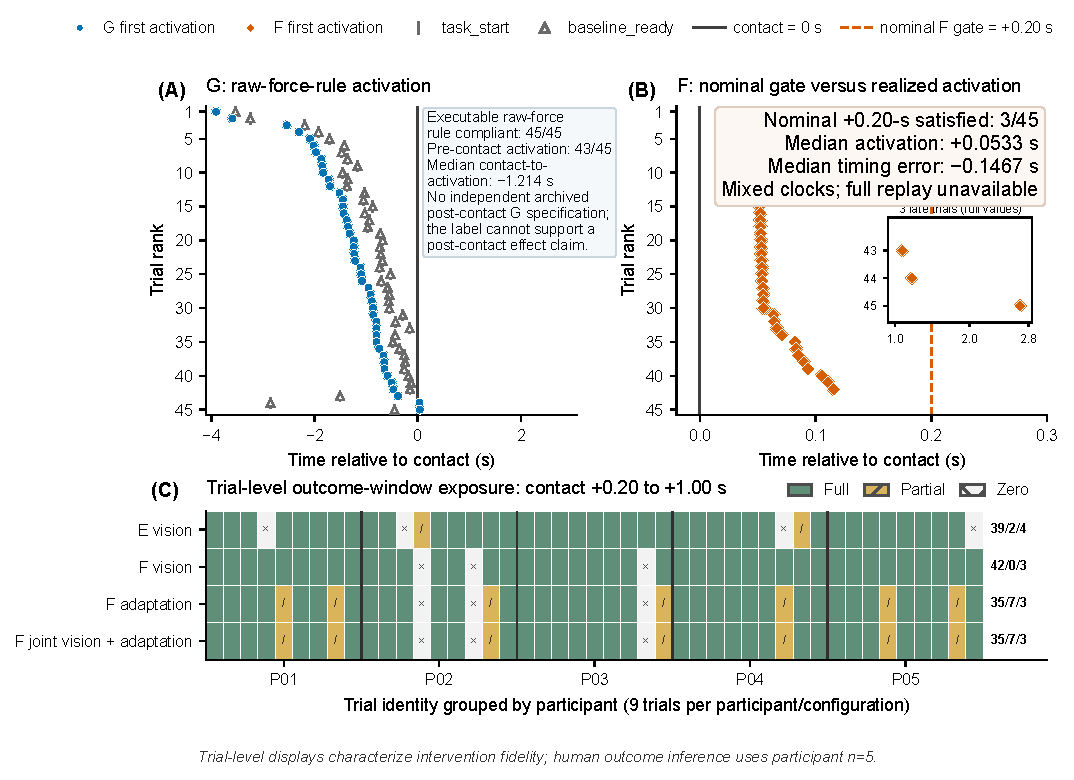
\includegraphics[width=0.98\textwidth]{Fig03_realized_intervention_fidelity_v5_1.pdf}
    \caption{Realized activation timing for G/F and outcome-window exposure
    for E/F. (A) Timing of the first G activation relative to contact and replay
    results for the executable rule. (B) Realized F activation relative to the
    nominal $+0.20$-s gate; the mixed clocks and unavailability of complete
    $C\rightarrow R$ predicate replay are explicitly marked. (C) Trial-level
    full, partial, and zero exposure for E/F during the post-contact
    0.20--1.00-s window. Human-outcome inference remains at the level of 5
    participants.}
    \label{fig:fidelity_results}
\end{figure*}

\subsection{RQ3: Comparison Identity After Reconstruction}

The evidence states and admissible interpretations are summarized in
Table~\ref{tab:comparison_identity}. Reconstruction neither excluded trials
nor regrouped them according to outcomes; it changed the scientific names
assigned to the original condition comparisons.

\begin{table*}[t]
\caption{Realized-Intervention Fidelity and Supportable Comparison Identities for the Archived Conditions}
\label{tab:comparison_identity}
\centering
\scriptsize
\begin{tabularx}{\textwidth}{@{}p{0.075\textwidth}p{0.075\textwidth}p{0.10\textwidth}p{0.12\textwidth}p{0.15\textwidth}Y@{}}
\toprule
Configuration & $s_N$ & $s_{NC}$ & $s_{CR}$ & Window exposure & Supportable identity and comparison boundary \\
\midrule
A & available & pass & pass & 45 full & Fixed A identity can be retained; causal interpretation is not automatically authorized \\
G & unavailable & not evaluable & pass & 40 full/5 partial & Replay-consistent realized original-force G versus fixed A; cannot be described as a purely post-contact effect \\
E & available & pass & pass & 39 full/2 partial/4 zero & Assigned bundled E configuration with heterogeneous visual exposure versus A; cannot be decomposed into isolated visual, stiffness, or force effects \\
F & available & fail: clock & not evaluable & 35 full/7 partial/3 zero & Recorded early/heterogeneous F versus E; cannot be described as the correctly implemented $+0.20$-s strategy or as establishing $C=R$ \\
\bottomrule
\end{tabularx}
\end{table*}

Consequently, G--A can describe only the realized original-force G rule,
predominantly activated before contact, relative to fixed A. E--A describes
assignment to the bundled E configuration and its heterogeneous visual
exposure relative to A. F--E describes the recorded early/heterogeneous F
configuration relative to E, with disclosure that complete delivery replay
was not evaluable. F--G likewise cannot be interpreted as factorial main
effects of vision, force, or their interaction.

\subsection{Exploratory Outcome Pattern Under the Retained Comparison}

For the E--A realized-configuration comparison that remained descriptively
supportable after reconstruction, the mean difference in operational
excess-force impulse was $-0.3489$~N$\cdot$s (95\% CI, $-0.6080$ to
$-0.0898$; paired t-test, $p=0.0201$); the difference was negative for all 5
participants. The exact sign-flip and Wilcoxon tests both yielded $p=0.0625$.
After Holm correction across 4 contrasts, the paired t-test yielded 0.0633 and
both exact tests yielded 0.2500. This result is therefore an exploratory,
directionally consistent pattern for the bundled E configuration, rather than
a confirmatory causal effect or an isolated mechanism.

Across all 64/64 record selections, the E--A mean remained negative, ranging
from $-0.353791$ to $-0.336697$~N$\cdot$s, and every selection retained
negative differences for all 5 participants. This robustness check neither
changed the provenance status of the erroneous initial records nor increased
the independent sample size.

\begin{figure*}[t]
    \centering
    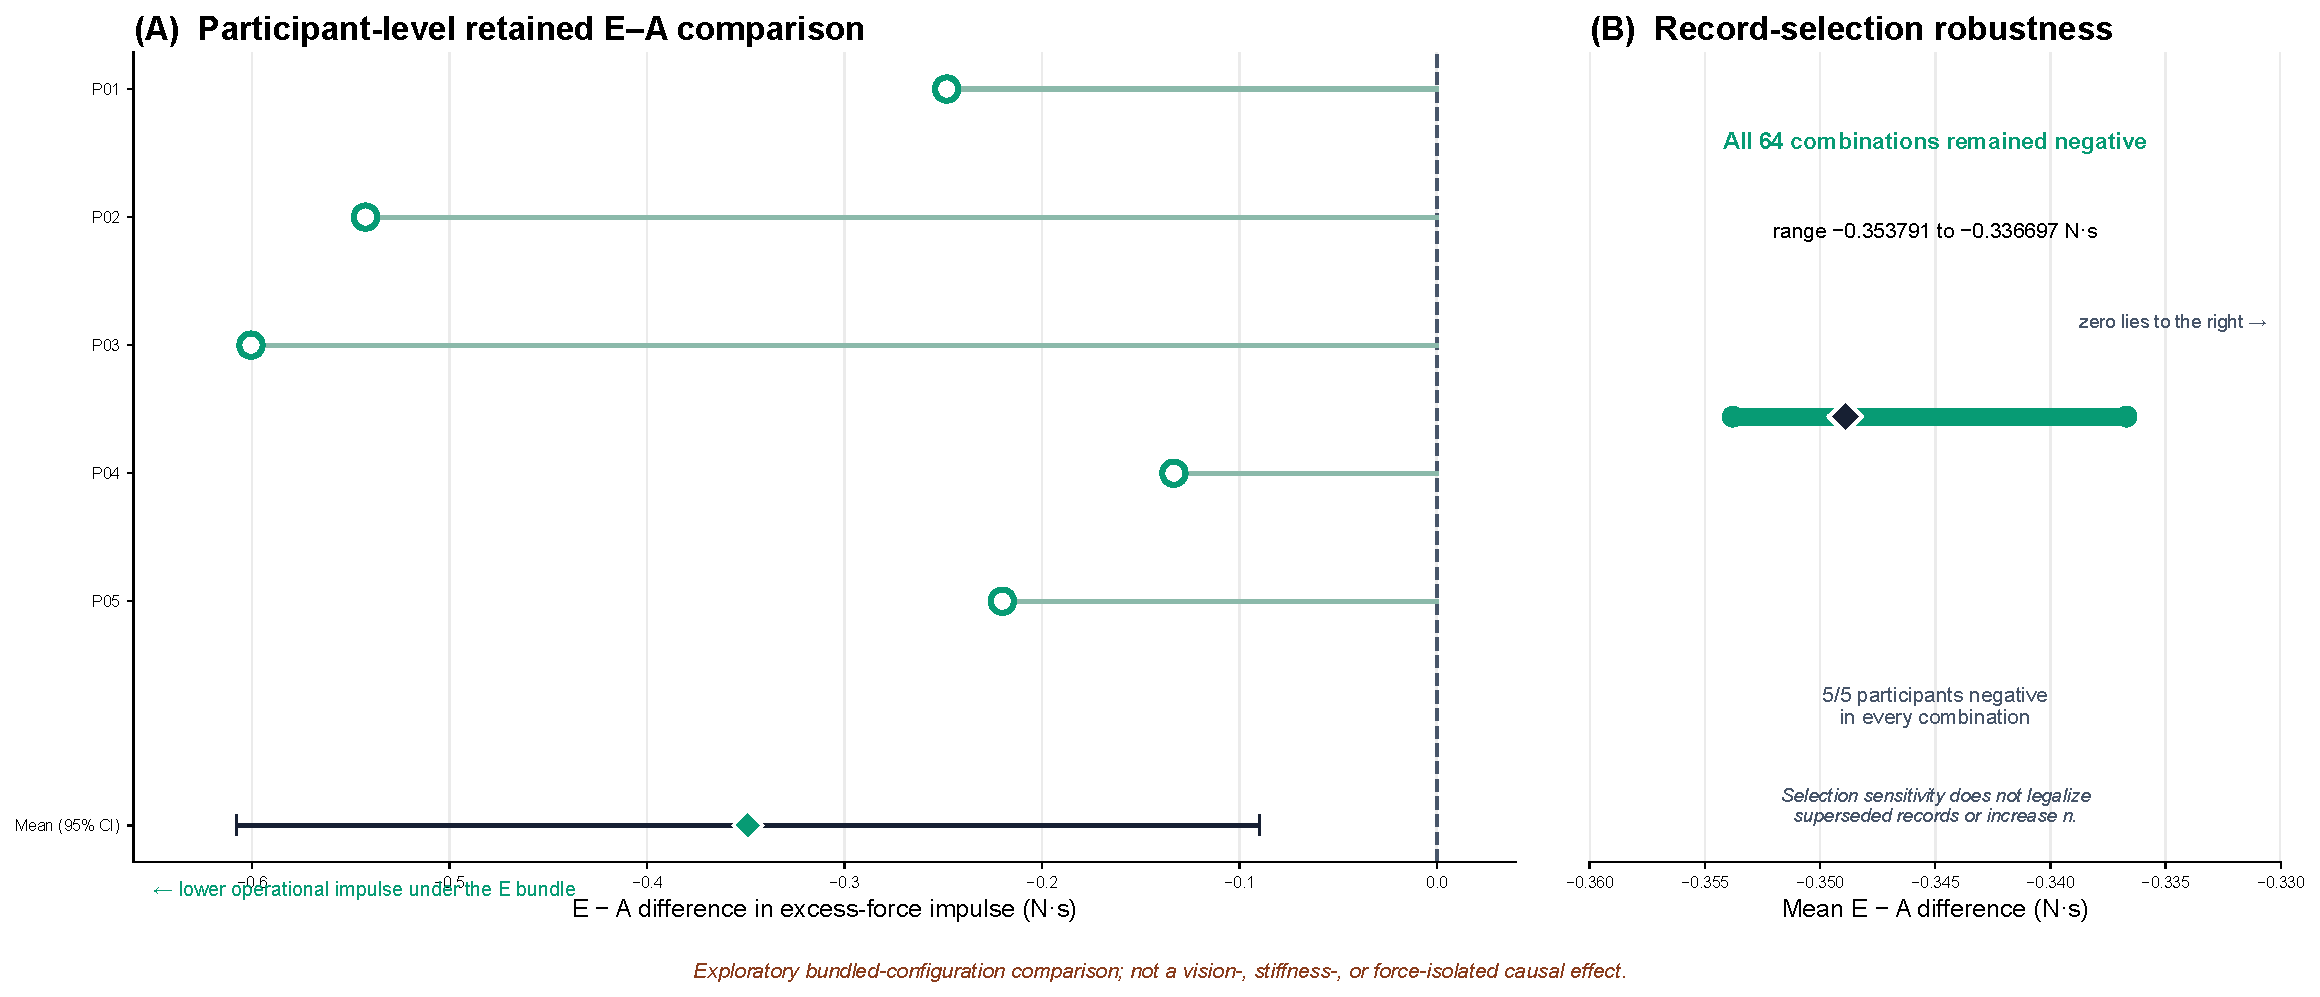
\includegraphics[width=0.90\textwidth]{Fig04_EA_outcome_robustness_v5_1.pdf}
    \caption{Participant-paired E--A outcomes and record-selection robustness.
    (A) Paired E--A differences in operational excess-force impulse during the
    post-contact 0.20--1.00-s window for 5 participants, with the 95\%
    confidence interval for the mean. (B) Range of the E--A mean across 64
    record selections. The comparison shown is between the bundled E
    configuration with heterogeneous visual exposure and fixed A; it does not
    represent a causal effect of an isolated visual, stiffness, or force
    strategy.}
    \label{fig:outcome}
\end{figure*}

\subsection{Rule-Level Internal Verification}

All 12/12 frozen cases returned the expected evidence states, cumulative
diagnoses, identities, and comparison levels. The checks confirmed that a
label cannot make a missing specification available, guard and clock
mismatches can coexist, and approximately 1~ms of exposure remains partial
exposure. They also confirmed that a missing trajectory produces unavailable
rather than zero exposure, invalid provenance prevents evaluation of the
intervention--outcome link, and incomplete replay can coexist with known
exposure. These results constitute rule-level implementation verification,
not diagnostic accuracy, a methodological validity rate, or external
validation.

Because the cases were constructed controls rather than a sample from a fault
population, 12/12 denotes complete agreement with the frozen oracle for this
test set, not an estimated success probability. Agreement at both the
intermediate-state and final-decision levels shows that the reported labels
can be regenerated through the declared transformation; it does not
independently validate author judgments about artifact sufficiency.

% ============================================================
\section{Discussion}
% ============================================================

\subsection{Implications for the Interpretation of Human--Machine Experiments}

The main finding is not a software defect itself. Rather, intervention delivery
timing and window exposure can change the closed loop entered by the operator.
G predominantly activated before contact, most F activations occurred earlier
than the nominal gate, and some E trials lacked full exposure to the visual
configuration during the outcome window. Each discrepancy could change the
machine state and feedback available to the operator during approach, contact,
and correction, thereby changing subsequent input and the outcome trajectory.
A condition label is therefore not a sufficient experimental unit for a
human--machine intervention.

Activation timing and window exposure answer related but non-equivalent
questions. Timing locates a state change within the closed-loop trajectory;
exposure quantifies the opportunity for that state to influence the predefined
outcome window. An intervention may activate before contact yet fully cover a
later window, or activate after contact and cover only part of it. Neither
quantity establishes that the operator consciously perceived the change; both
describe recorded properties of the delivered human--machine configuration.

Realized-intervention reconstruction also changed the scientific identity of
the results. The available data cannot answer questions about a purely
post-contact G intervention, a correctly gated F intervention, or a factorial
vision-by-force effect. They can still address a narrower question: what
descriptive differences are observed between a particular archived
implementation, with its recorded exposure distribution, and a fixed or other
realized configuration? This narrowing does not exclude unfavorable trials. It
aligns the comparison name with verifiable evidence.

\subsection{Requirements for Prospective Experimental Design}

Prospective asynchronous human--machine experiments should freeze the
intervention specification, common clock, event definitions, outcome window,
and independent experimental unit before acquisition. During acquisition,
they should preserve every guard input, the reason for each state transition,
the complete activation trajectory, and exact record identity. Evidence
reconstruction should be conducted independently before inference. Reports
should present the nominal assignment, realized delivery timing, exposure
distribution, and any element that was not evaluable.

These requirements do not replace evaluations of control performance,
usability, workload, or subjective experience. Instead, they establish a
credible treatment identity for those measures. Particularly in systems that
update visual, haptic, and control parameters asynchronously, delivery and
exposure should be recorded as experimental variables rather than embedded as
implementation assumptions within condition labels.

A minimum prospective evidence package therefore includes a machine-readable
nominal specification, explicit guard inputs and clock domains, transition
causes, complete state trajectories, immutable trial identifiers and hashes,
and a frozen outcome-window definition. The interpretation rules should also
be fixed before outcome inspection. This package makes a failed link visible
at the point where it occurs and permits a narrower claim to survive when the
available evidence still supports one.

\subsection{Methodological Implications}

The framework connects several previously separate lines of work. Latency
research shows that timing may affect human--machine performance; runtime
verification checks software properties; reproducibility research preserves
artifacts and procedures; implementation fidelity distinguishes a planned
intervention from its implementation; and estimand research links theory to
statistics. HRI experiment-design and measurement work provides complementary
guidance on logging, reporting, and outcome constructs
\cite{hoffmanZhao2020,steinfeld2006,hoffman2019}, while formal HRI and rosbag
reliability studies reinforce the need for verifiable system properties and
temporally aligned records \cite{kressGazit2021,vigni2024}. The contribution
of this study is to transform this evidence into comparison identities and
wording boundaries, while preserving the
distinctions between automated computation and semantic audit, trial-level
fidelity and participant-level inference, and identity verification and causal
identification.

The framework is most useful for stateful, event-triggered, multiprocess, or
otherwise asynchronous interventions whose delivery can vary within an
analysis window. A reduced evidence chain may suffice for a synchronous fixed
command that is observed directly. In neither setting can fidelity
reconstruction recover undocumented intent, create randomization, remove
confounding, infer subjective perception, or identify the component effects
of bundled interventions.

The 12 controlled cases make the rule implementation executable and
challengeable by counterexamples, but they do not establish that the rule
space is complete. The archived case shows that multiple discontinuities can
coexist within one acquisition; it does not constitute cross-system external
validation. Future methodological validation should prospectively freeze
specifications and oracles across multiple platforms, inject known and unknown
faults through an independent process, and evaluate diagnostic accuracy, rates
of not-evaluable determinations, and semantic-audit agreement.

\subsection{Limitations}

The independent human sample comprised only 5 participants, and the framework
was operationalized in only one archived teleoperation system. Information
about prospective randomization or counterbalancing was not recovered. E and
F were bundled multiparameter configurations; E--A and F--E cannot be
attributed to isolated visual, stiffness, force-feedback, or gripper
parameters. Contact alignment and the outcome shared the Panda internal force
estimate, and logged stiffness was not an independently measured physical
impedance.

Participant demographics, training, object geometry, and several
experimental-procedure details were not recovered from the current record
lineage. The structured semantic audit was author-conducted and did not use
independent dual coding. Complete cycle-level predicate inputs for F were
unavailable, so the complete $C\rightarrow R$ relation could only be recorded
as not evaluable. Contemporaneous evidence for the failure of 6 replaced
record groups remained incomplete; the 64 combinations cannot make erroneous
records provenance-valid. Ethics approval or exemption and informed consent
must be resolved affirmatively from contemporaneous institutional records
before submission.

% ============================================================
\section{Conclusion}
% ============================================================

Nominal condition labels alone do not establish that an asynchronous
human--machine system delivered the corresponding intervention in the
operator--machine loop. By linking the specification, implementation,
trial-level delivery, window exposure, and record identity,
realized-intervention fidelity reconstruction determines when a nominal
comparison can be retained, when it must be recast, and when it is not
evaluable. In this archived teleoperation case, the process materially changed
the scientific identities of comparisons involving G, E, and F and constrained
E--A to an exploratory bundled-configuration comparison. Future human--machine
experiments should record intervention delivery timing and window exposure as
explicit experimental variables so that ``what was actually compared'' can be
verified before statistical inference.

\begingroup
\sloppy
\hfuzz=1pt
\bibliographystyle{IEEEtran}
\bibliography{references}
\endgroup

\end{document}
